\subsection{Live MEAM Evaluation App}
\label{sec:meam_app}

The optimized twelve-element library is also exposed through a small
LAMMPS-backed web app that runs the elastic-property protocol of
Section~\ref{sec:stage2} against it on demand. A composition and a few box and
run-length knobs go in, a real strain sweep runs, and the app reports
$C_{11}$, $C_{12}$, the derived $E$ and $\nu$, and whether the result passes
the Born stability check. Each run is keyed by a
hash of its inputs and cached, and the cache is invalidated whenever the MEAM
file changes, so re-running a composition after a refit recomputes rather than
returning a stale number. Figure~\ref{fig:meam_app} shows the interface on a
pure-aluminium run.

\begin{figure}[htbp]
	\centering
	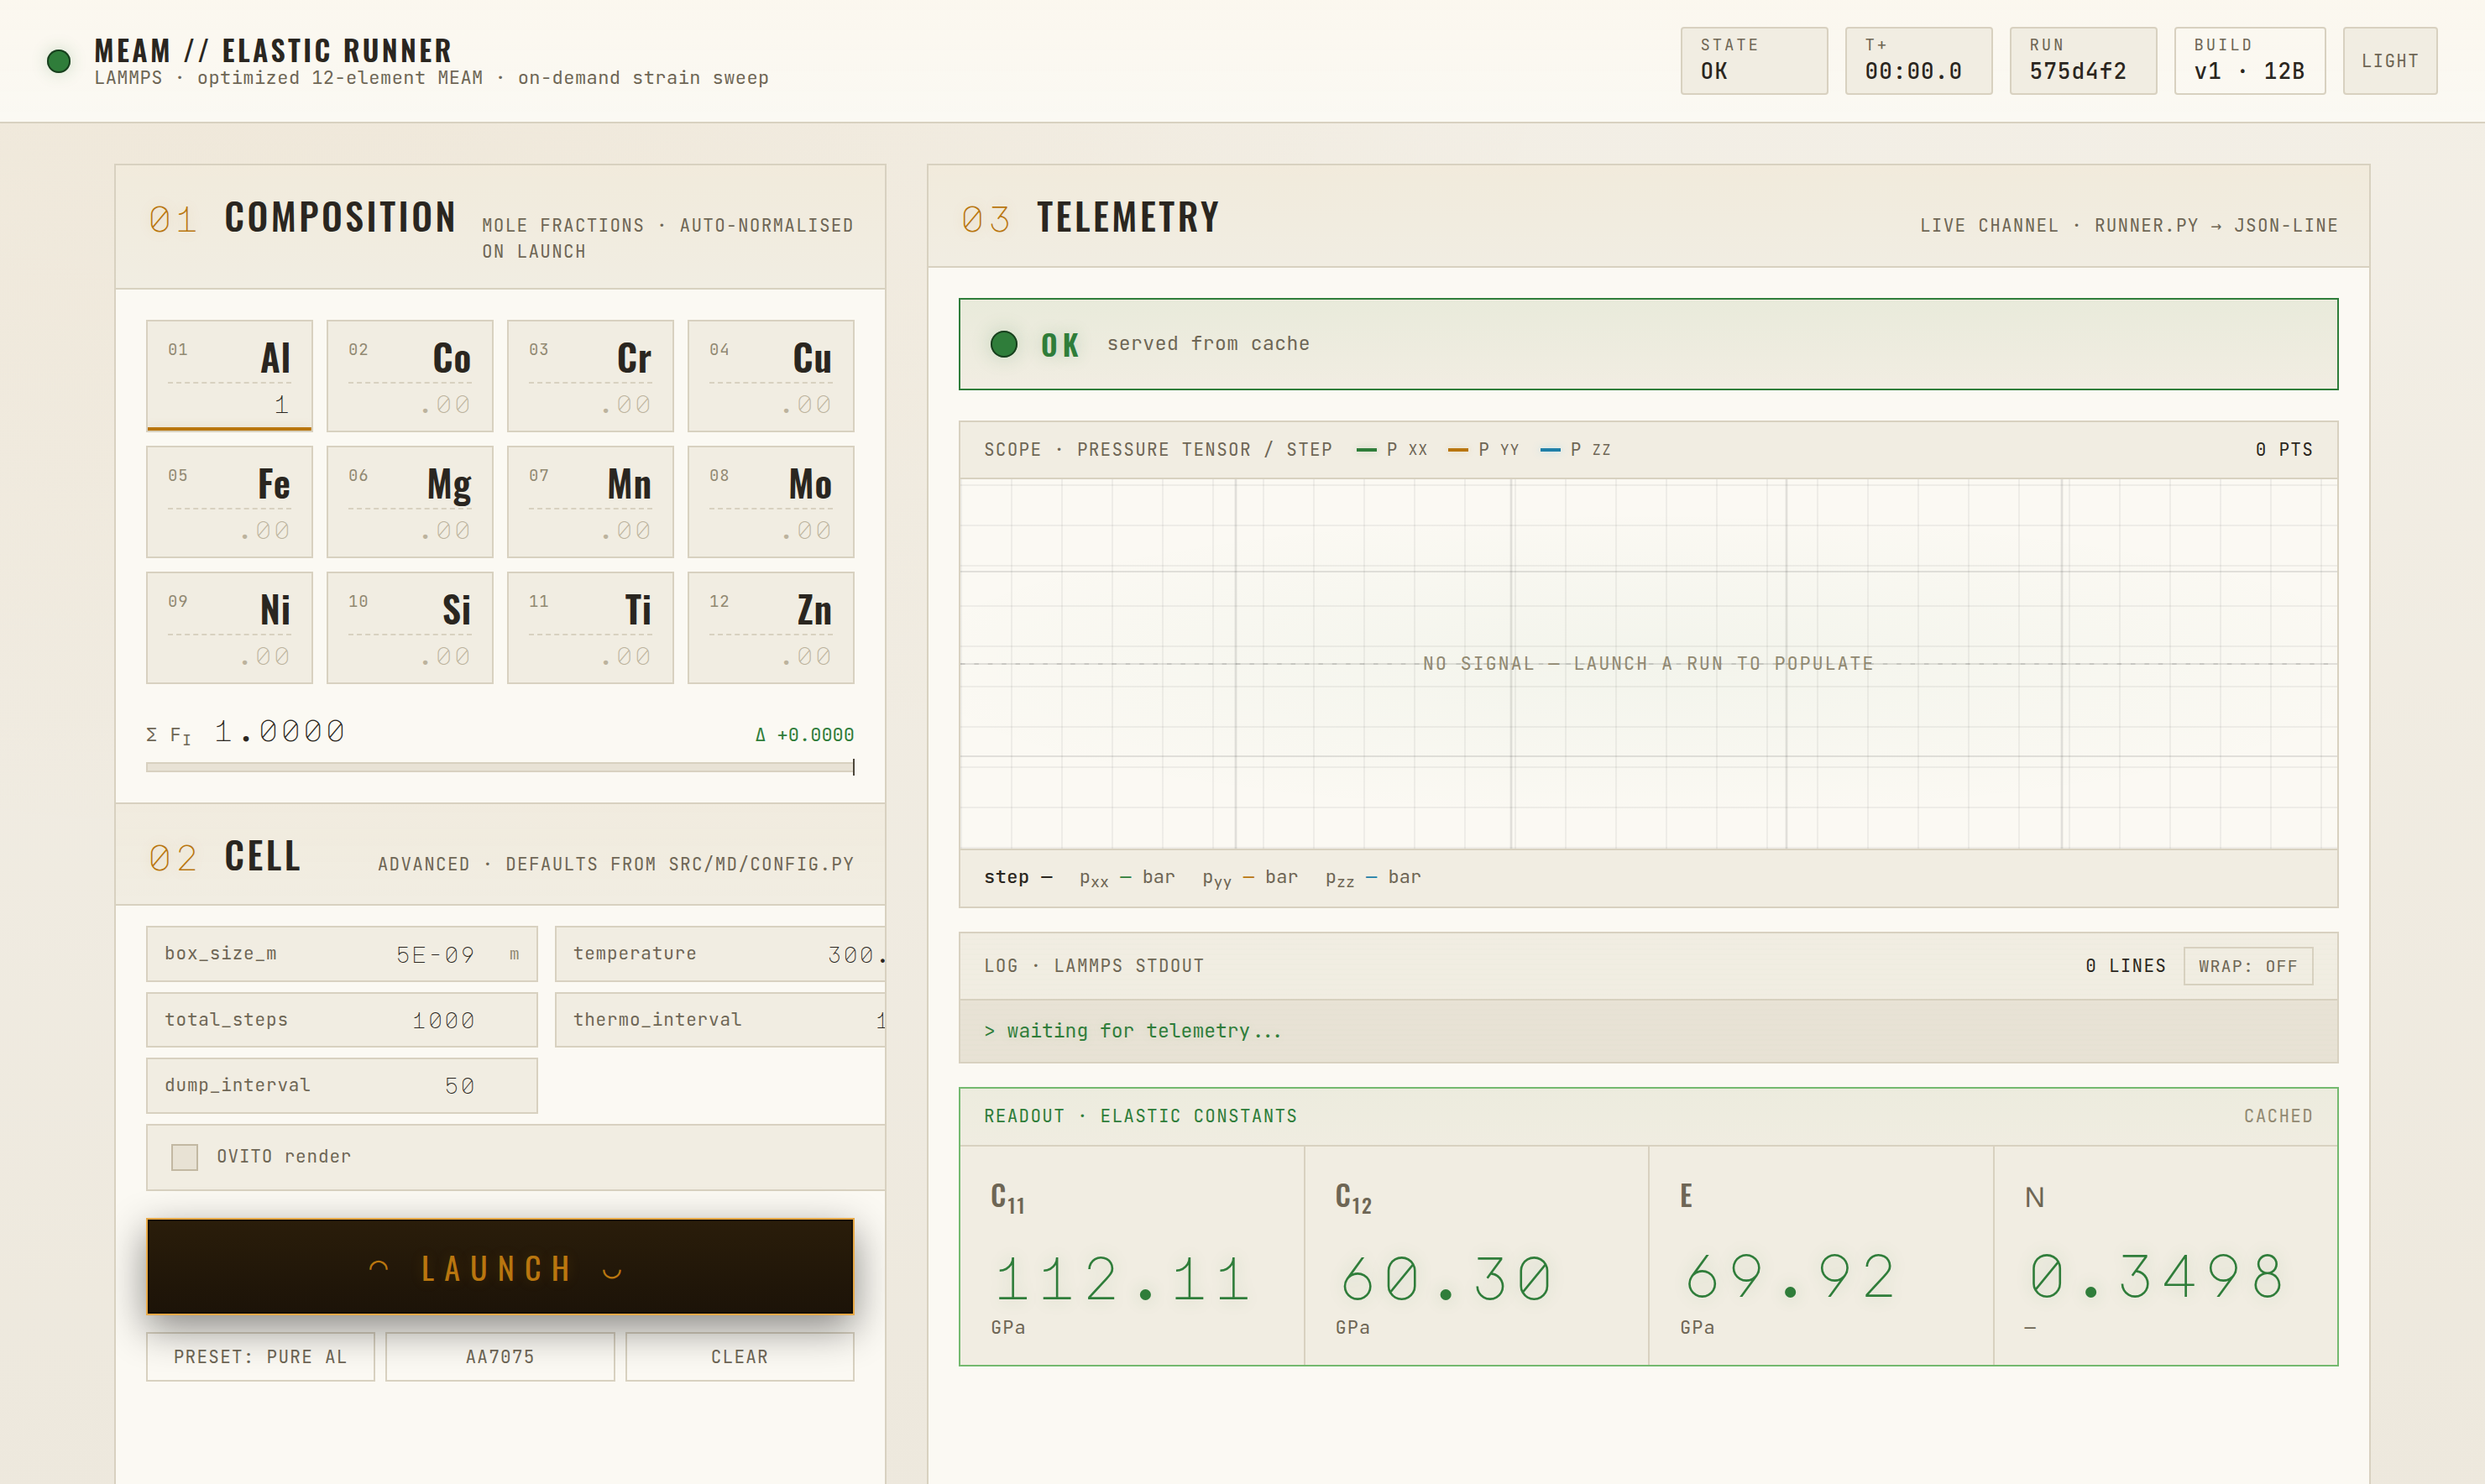
\includegraphics[width=0.95\textwidth]{figures/meam_app_light.png}
	\caption{The MEAM elastic-runner app, shown on a pure-aluminium run against
	the optimized potential. The left column sets the composition and the
	supercell and run-length knobs; the right column streams the LAMMPS job and
	reports the elastic-constants readout. Here the run returns
	$C_{11}=112.1$\,GPa, $C_{12}=60.3$\,GPa, $E=69.9$\,GPa, and $\nu=0.350$.}
	\label{fig:meam_app}
\end{figure}

The pure-aluminium numbers are a useful sanity check on the optimized
potential. Polycrystalline aluminium sits near $E=70$\,GPa with
$\nu\approx0.33$ to $0.35$ in handbook data, and the optimized MEAM returns
$E=69.9$\,GPa and $\nu=0.350$, essentially on top of the experimental value.
The cubic constants themselves, $C_{11}=112.1$ and $C_{12}=60.3$\,GPa, differ
from the DFT single-crystal values of Table~\ref{tab:dft_elements}
($167.1$ and $32.6$\,GPa), which is expected: the potential was refit to the
MD elastic targets that drive the whole pipeline, not to the DFT single-crystal
tensor, and the two protocols probe the response differently. The app makes
that distinction inspectable, since any composition the optimized library
covers can be run and compared against a reference on the spot.
